\chapter{Waterstof en het s-blok}\label{ch:b1:s-block}

Elke telefoon, laptop en elektrische auto heeft een batterij waarin de
positieve ladingen door lithiumionen gedragen worden. Dat lithium komt
vooral van twee plaatsen: mijnen in hard gesteente in Australië en de
zoutvlakten van de Andes, waar pekel die van onder de korst opgepompt
wordt maandenlang in de zon verdampt, tot er lithiumzouten uit neergeslagen
kunnen worden. Lithium is het eerste van de \omterm{def:b1:s-block:families}{alkalimetalen}, de reactiefste
metalen die er bestaan, en zijn buren natrium, kalium, magnesium en
calcium leveren de basischemicaliën van de industrie: bijtende soda,
soda, kalk. Dit hoofdstuk opent de beschrijvende chemie van de elementen
met waterstof en het \omterm{def:b1:periodicity:table}{s-blok}, en gebruikt de werktuigen van de vorige
hoofdstukken --- ionisatie-energieën, \omterm{def:b1:nernst:electrode-potential}{standaardpotentialen},
\omterm{def:b1:precipitation:solubility-product}{oplosbaarheidsproducten} --- om te verklaren wat deze elementen doen.

\begin{recall}
Ionisatie-energieën en \omterm{def:b1:periodicity:electronegativity}{elektronegativiteit} (\cref{ch:b1:periodicity});
\omterm{def:b1:nernst:electrode-potential}{standaardpotentialen} (\cref{ch:b1:nernst}); \omterm{def:b1:precipitation:solubility-product}{oplosbaarheidsproducten} en
het neerslaan van hydroxiden (\cref{ch:b1:precipitation}). Het schoolboek
(jaar 10) deelde de elementen in families in: \omterm{def:b1:s-block:families}{alkalimetalen},
\omterm{def:b1:s-block:families}{aardalkalimetalen}, halogenen, edelgassen.
\end{recall}

\begin{omfigure}
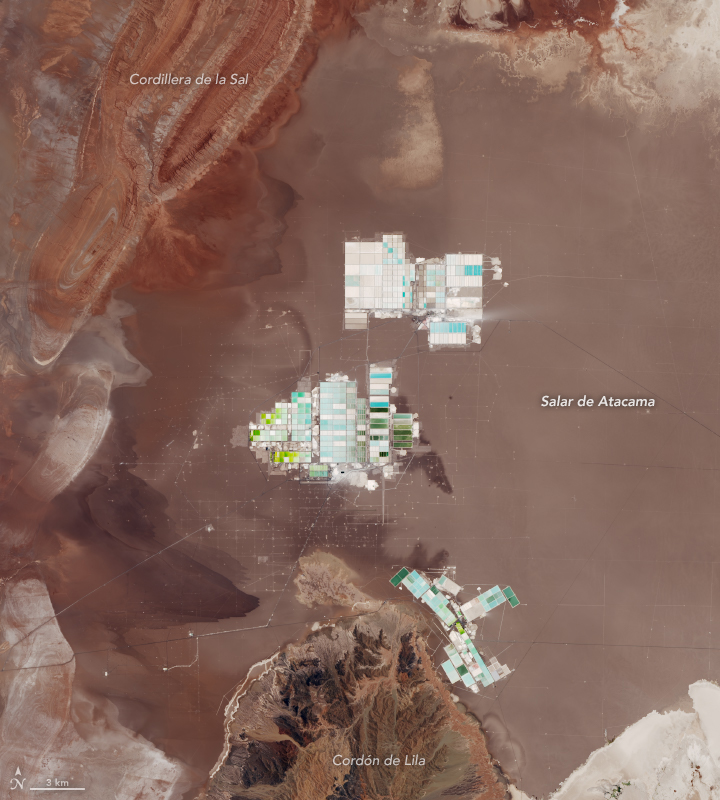
\includegraphics[width=0.48\linewidth]{images/book2/atacama-ponds.jpg}

{\small Verdampingsbekkens met lithiumpekel op de Salar de Atacama, gezien
vanuit een baan om de aarde (Landsat 8, 2018; NASA Earth Observatory,
publiek domein, Wikimedia Commons). De kleur van elk bekken verandert
naarmate de pekel geconcentreerder wordt en zouten kristalliseren.}
\end{omfigure}

\section{Waterstof en de hydriden}

Waterstof heeft één elektron: het kan dat afstaan (\ce{H+}, in water
gedragen als \ce{H3O+}), delen (\omterm{def:b1:lewis-resonance-vsepr:lewis}{covalente bindingen}), of er een opnemen
(\ce{H-}, met de \omterm{def:b1:quantum-numbers:configuration}{elektronenconfiguratie} van helium). Wat het doet, hangt
af van zijn partner.

\begin{definition}[Hydriden]\label{def:b1:s-block:hydride}
Een \emph{hydride}\index{hydride} is een binaire verbinding van waterstof
met een ander element. \emph{Zoutachtige hydriden}\index{zoutachtig hydride},
gevormd met de \omterm{def:b1:s-block:families}{alkalimetalen} en de zwaardere \omterm{def:b1:s-block:families}{aardalkalimetalen}
(\ce{LiH}, \ce{NaH}, \ce{CaH2}), zijn ionaire vaste stoffen die \ce{H-}
bevatten. \emph{Covalente hydriden}\index{covalent hydride}, gevormd met
de elementen van het \omterm{def:b1:periodicity:table}{p-blok} (\ce{CH4}, \ce{NH3}, \ce{H2O}, \ce{HCl}), zijn
moleculair. \emph{Metallische hydriden}\index{metallisch hydride},
gevormd met sommige overgangsmetalen, zijn vaste stoffen waarin waterstof
\omterm{def:b1:crystals-metals:site}{interstitiële holten} van het \omterm{def:b1:crystals-metals:lattice}{rooster} van het metaal bezet, vaak met een
variabele samenstelling.
\end{definition}

Het hydride-ion is een zeer \omterm{def:b1:predominant-reaction:strong-acid}{sterke base} en een sterke \omterm{def:b1:nernst:couple}{reductor}:
\omterm{def:b1:s-block:hydride}{zoutachtige hydriden} reageren met water, \ce{NaH + H2O -> NaOH + H2}, en
dienen als droogmiddel voor oplosmiddelen en als base in de organische
synthese (\cref{ch:b1:alcohol-activation}). De \omterm{def:b1:s-block:hydride}{covalente hydriden} van de
tweede \omterm{def:b1:periodicity:table}{periode} tonen het verloop van de \omterm{def:b1:periodicity:electronegativity}{elektronegativiteit} door die
\omterm{def:b1:periodicity:table}{periode} heen: \ce{CH4} zuur noch basisch, \ce{NH3} basisch, \ce{H2O}
amfoteer, \ce{HF} zuur.

\section{De alkalimetalen}

\begin{definition}[Alkalimetalen en aardalkalimetalen]\label{def:b1:s-block:families}
De \emph{alkalimetalen}\index{alkalimetaal} (Li, Na, K, Rb, Cs, Fr) vormen
\omterm{def:b1:periodicity:table}{groep} 1, met één valentie-elektron \textit{ns}$^1$; de
\emph{aardalkalimetalen}\index{aardalkalimetaal} (Be, Mg, Ca, Sr, Ba, Ra)
vormen \omterm{def:b1:periodicity:table}{groep} 2, met \textit{ns}$^2$. Hun elementen vormen het \omterm{def:b1:periodicity:table}{s-blok}.
\end{definition}

\begin{proposition}[De alkalimetalen zijn sterke reductoren]\label{prop:b1:s-block:reducing-power}
De \omterm{def:b1:s-block:families}{alkalimetalen} hebben de laagste eerste ionisatie-energieën van hun
\omterm{def:b1:periodicity:table}{periode} (Li \qty{5.39}{eV}, Na 5.14, K 4.34) en zeer negatieve
\omterm{def:b1:nernst:electrode-potential}{standaardpotentialen} (\ce{Li+}/\ce{Li} $-3.04$~V, \ce{Na+}/\ce{Na}
$-2.71$, \ce{K+}/\ce{K} $-2.94$): ze reduceren water en komen in de natuur
alleen voor als \ce{M+}-ionen.
\end{proposition}
% ledger: ie:Li, ie:Na, ie:K (E0 computed in figdata/bachelor-1/standard-potentials.py)

\begin{proof}
Eén enkel elektron buiten een edelgaskern, ver van de kern en afgeschermd
door de binnenste schillen (\cref{ch:b1:periodicity}), is gemakkelijk te
verwijderen. In water is het kleine \ce{M+}-ion sterk gehydrateerd, wat
de potentiaal van het koppel nog verlaagt. Met een $E^\circ$ die meer dan
\qty{2.2}{V} onder de lijn van water bij pH 7 ($-0.41$~V) ligt, heeft de
reactie \ce{2M + 2H2O -> 2M+ + 2OH- + H2} een enorme constante
(\cref{prop:b1:nernst:equilibrium-constant}).
\end{proof}

\begin{omfigure}
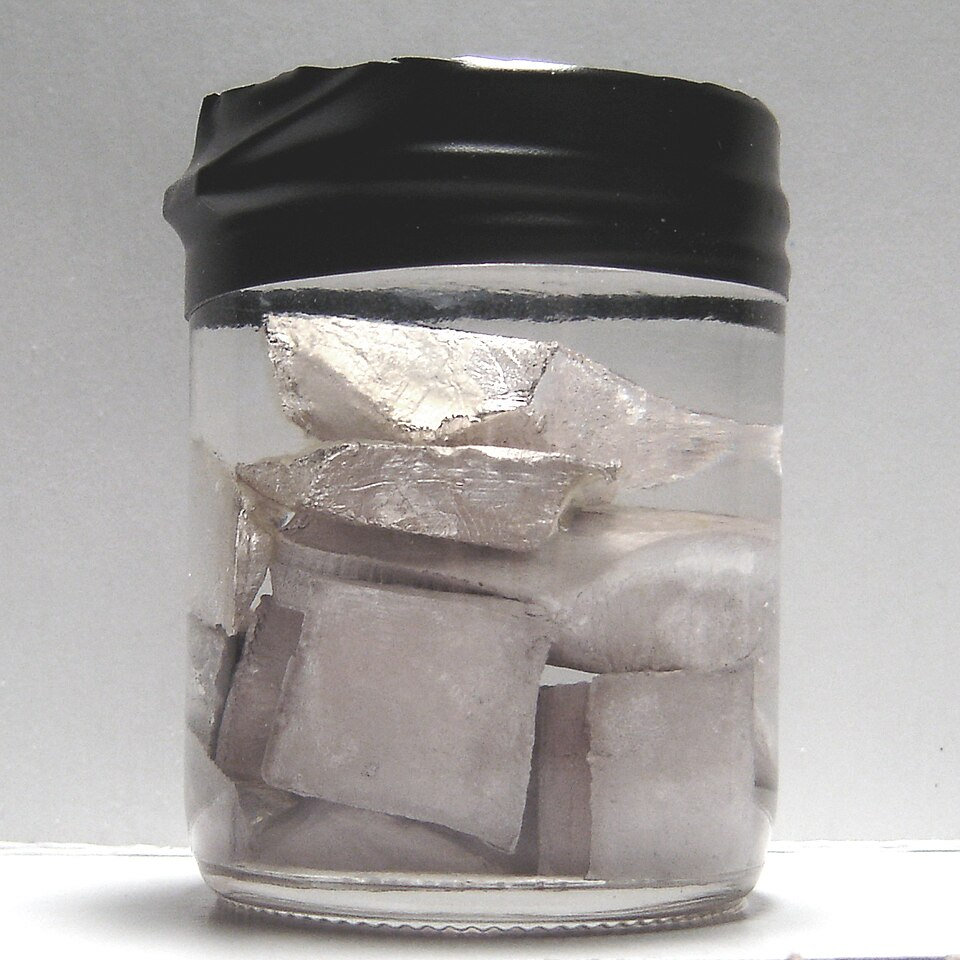
\includegraphics[height=4.6cm]{images/book2/sodium-oil.jpg}\hspace{0.8em}%
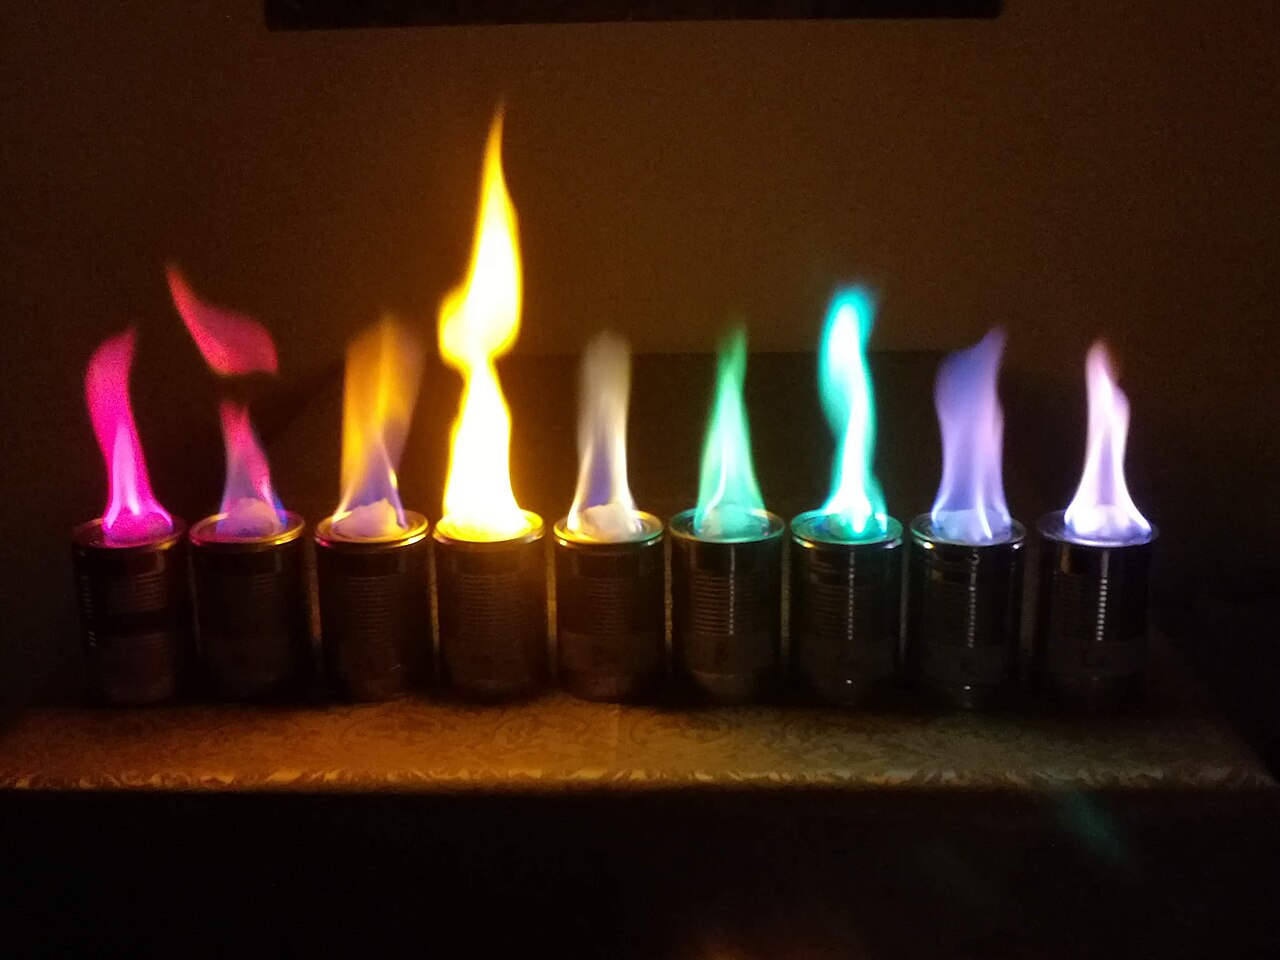
\includegraphics[height=4.6cm]{images/book2/flame-colours.jpg}

{\small Links: natrium wordt onder minerale olie bewaard, weg van lucht en
vocht (foto Justin Urgitis, CC BY-SA 2.5). Rechts: vlamkleuren, van links
naar rechts, van verbindingen van lithium, strontium, calcium, natrium,
barium, boor, koper, cesium en kalium: elektronen die in de vlam
aangeslagen worden, vallen terug naar lagere niveaus en zenden daarbij
licht uit met golflengten die kenmerkend zijn voor elk element
(\cref{ch:b1:quantum-numbers}) (foto Hegelrast, CC BY-SA 4.0). Beide
Wikimedia Commons.}
\end{omfigure}

\begin{inthelab}[Een demonstratie, geen experiment]
De reactie van natrium met water wordt alleen door een leraar getoond,
achter een veiligheidsscherm, met een stukje ter grootte van een linze
dat in een grote bak water met fenolftaleïne gegooid wordt: het metaal
smelt tot een rondrennend bolletje, waterstof bruist op, en het roze spoor
toont het gevormde hydroxide. Kalium ontsteekt de waterstof. Grotere
stukken ontploffen. Natrium wordt onder olie gesneden, met een tang
gehanteerd, en zijn resten worden met ethanol vernietigd, nooit met
water.
\end{inthelab}

Lithium is de uitzondering in zijn groep: het kleinste ion, het sterkst
gehydrateerd, dus de meest negatieve potentiaal, en toch reageert het het
traagst met water. Zijn verbindingen lijken op die van magnesium
(lithiumcarbonaat en -fosfaat zijn slecht oplosbaar, net als die van
magnesium), een diagonaalverwantschap in het periodiek systeem. De
\omterm{def:b1:s-block:families}{alkalimetalen} worden geproduceerd door elektrolyse van hun gesmolten
chloriden, omdat geen enkele chemische \omterm{def:b1:nernst:couple}{reductor} sterk genoeg is; de
elektrodereacties van zulke cellen worden in het deel van jaar~2
bestudeerd.

\section{Natriumverbindingen in de industrie}

\begin{definition}[Karakter van oxiden]\label{def:b1:s-block:oxide-character}
Een \emph{basisch oxide}\index{basisch oxide} reageert met water tot een
hydroxide, of met zuren tot zouten (\ce{Na2O}, \ce{CaO}); een \emph{zuur
oxide}\index{zuur oxide} reageert met water tot een zuur, of met basen
tot zouten (\ce{CO2}, \ce{SO3}, \ce{P4O10}); een \emph{amfoteer
oxide}\index{amfoteer oxide} reageert zowel met zuren als met basen
(\ce{Al2O3}, \ce{ZnO}). Door een \omterm{def:b1:periodicity:table}{periode} heen gaan de oxiden van basisch
(metalen, links) naar zuur (niet-metalen, rechts).
\end{definition}

Natriumhydroxide wordt gemaakt door elektrolyse van pekel (de
chlooralkali-elektrolyse, die ook chloor en waterstof oplevert).
Natriumcarbonaat, soda, gebruikt voor glas, wasmiddelen en de winning van
lithium, wordt ofwel als het mineraal trona gedolven, ofwel gemaakt uit
zout en kalksteen: in 2025 produceerde de wereld ongeveer 71 miljoen ton,
19 miljoen uit natuurlijke afzettingen en 52 miljoen synthetisch, het
meeste via het solvayproces.
% ledger: usgs:sodaash-total-2025, usgs:sodaash-natural-2025, usgs:sodaash-synthetic-2025

\begin{proposition}[Het solvayproces]\label{prop:b1:s-block:solvay}
Het solvayproces zet natriumchloride en calciumcarbonaat om in
natriumcarbonaat en calciumchloride, \ce{2NaCl + CaCO3 -> Na2CO3 +
CaCl2}, via stappen waarin ammoniak en koolstofdioxide gerecycleerd
worden.
\end{proposition}

\begin{proof}
De stappen zijn: (1) \ce{CaCO3 -> CaO + CO2} (kalkoven); (2) \ce{NaCl + NH3 +
CO2 + H2O -> NaHCO3 + NH4Cl} (carbonatatie van ammoniakale pekel; het
waterstofcarbonaat, het minst oplosbare zout dat aanwezig is, slaat
neer); (3) \ce{2NaHCO3 -> Na2CO3 + CO2 + H2O} (calcinering); (4) \ce{CaO + H2O ->
Ca(OH)2}; (5) \ce{Ca(OH)2 + 2NH4Cl -> CaCl2 + 2NH3 + 2H2O} (terugwinning
van ammoniak). Tel je $(1) + 2\times(2) + (3) + (4) + (5)$ op, dan vallen
\ce{NH3}, \ce{CO2}, \ce{NH4Cl}, \ce{NaHCO3}, \ce{CaO}, \ce{Ca(OH)2} en
water weg: \ce{2NaCl + CaCO3 -> Na2CO3 + CaCl2}.
\end{proof}

\begin{omfigure}
\begin{tikzpicture}[font=\small, >={Stealth}, box/.style={draw, rounded corners, fill=omDef!8, minimum width=2.6cm, minimum height=0.8cm, align=center}]
  \node[box] (kiln) at (0,0) {kalkoven\\\ce{CaCO3 -> CaO + CO2}};
  \node[box] (tower) at (5.3,0) {carbonatatietoren\\\ce{NaHCO3} slaat neer};
  \node[box] (calc) at (10.2,0) {calcineeroven\\\ce{NaHCO3} $\to$ \ce{Na2CO3}};
  \node[box] (slake) at (0,-2.6) {kalkblusser\\\ce{CaO + H2O -> Ca(OH)2}};
  \node[box] (still) at (5.3,-2.6) {ammoniakkolom\\\ce{NH4Cl + Ca(OH)2}};
  \draw[->, thick] (kiln) -- node[above] {\ce{CO2}} (tower);
  \draw[->, thick] (tower) -- node[above, font=\scriptsize] {\ce{NaHCO3}} (calc);
  \draw[->, thick] (calc.north) -- ++(0,0.6) -| node[pos=0.25, above] {\ce{CO2} gerecycleerd} (tower.north);
  \draw[->, thick] (kiln) -- node[left] {\ce{CaO}} (slake);
  \draw[->, thick] (slake) -- node[above, font=\scriptsize] {\ce{Ca(OH)2}} (still);
  \draw[->, thick] (tower) -- node[right] {\ce{NH4Cl}} (still);
  \draw[->, thick] (still.east) -- ++(1.2,0) |- node[pos=0.25, right] {\ce{NH3} gerecycleerd} ($(tower.east)+(0,-0.25)$);
  \draw[<-, thick] (tower.north west) -- ++(-0.5,0.6) node[above] {pekel \ce{NaCl}};
  \draw[->, thick] (calc.east) -- ++(0.8,0) node[right] {\ce{Na2CO3}};
  \draw[->, thick] (still.south) -- ++(0,-0.6) node[below] {\ce{CaCl2}};
\end{tikzpicture}

{\small Het solvayproces. Koolstofdioxide en ammoniak circuleren in
kringlopen; zout en kalksteen gaan erin, soda en calciumchloride komen
eruit.}
\end{omfigure}

\begin{omfigure}
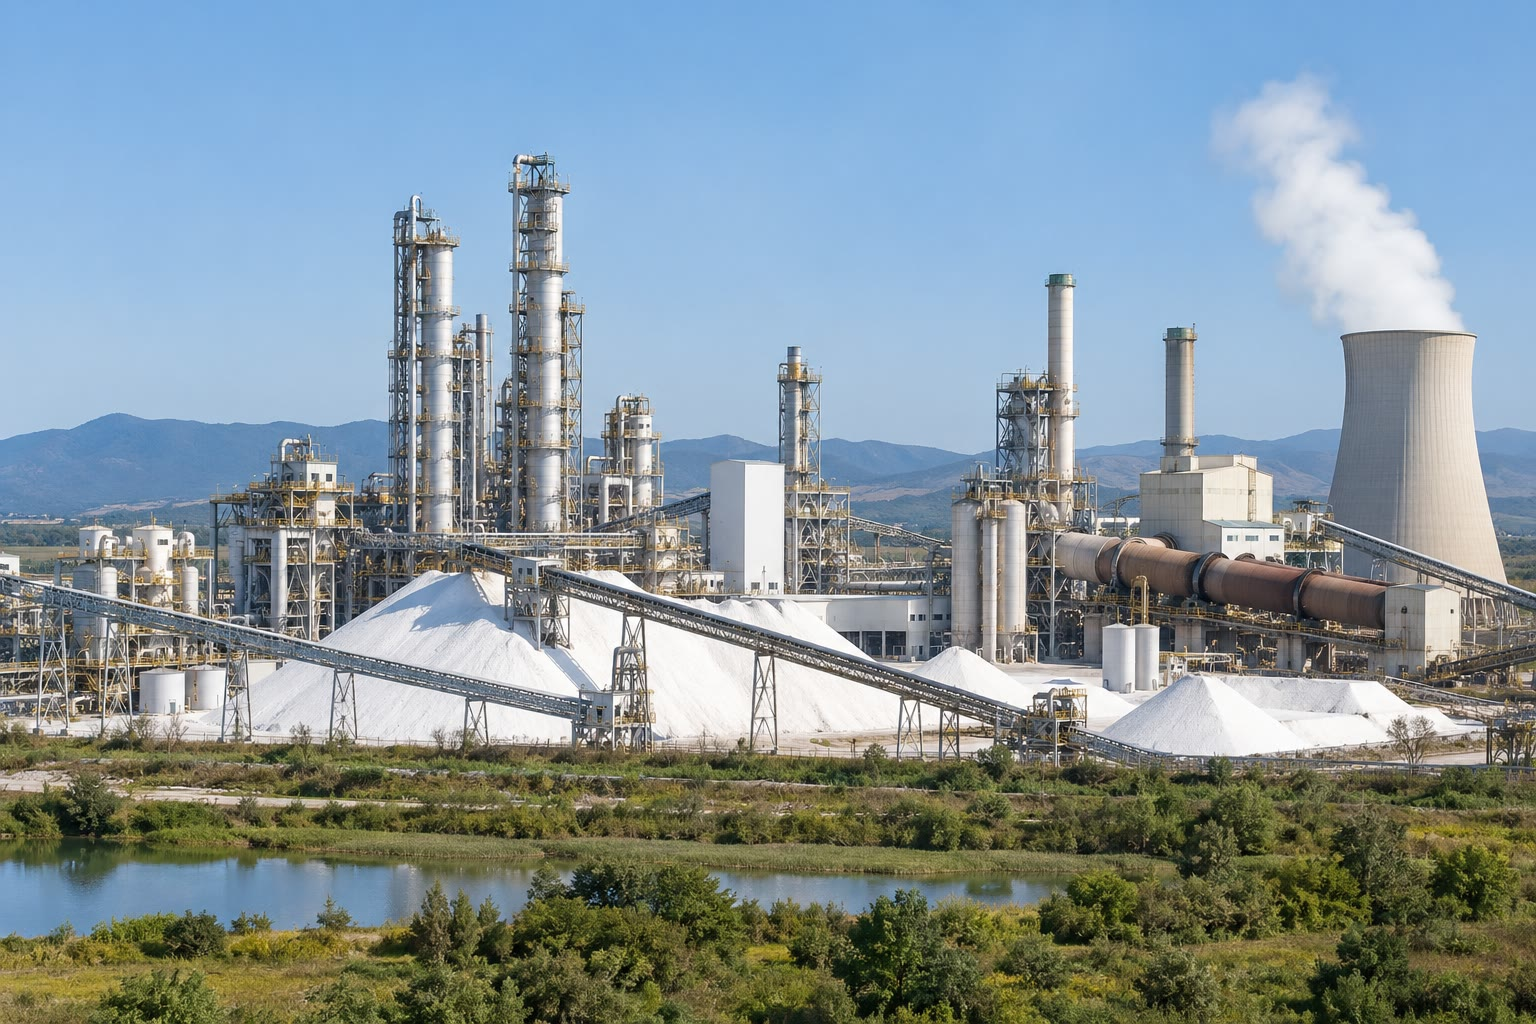
\includegraphics[width=0.55\linewidth]{images/book2/ai/b1-26-soda-ash-plant.jpg}

{\small Een sodafabriek: kalkovens, carbonatatietorens en voorraadbergen
natriumcarbonaat.}
\end{omfigure}

\begin{method}[Massabalans op een processchema]\label{met:b1:s-block:mass-balance}
\begin{enumerate}
  \item Schrijf de totale vergelijking op (som van de stappen, met de
        gerecycleerde deeltjes weggestreept).
  \item Bereken vanuit het gewenste product de hoeveelheden grondstoffen
        met de totale vergelijking, en corrigeer daarna voor het \omterm{def:b1:extent-q-and-k:fractional-extent}{rendement}
        van elke stap.
  \item Bereken voor een gerecycleerd deeltje alleen de aanvulling die
        nodig is om zijn verliezen te vervangen.
  \item Controleer de balans van elk element tussen invoer en uitvoer.
\end{enumerate}
\end{method}

\section{De aardalkalimetalen}

Magnesium en calcium zijn minder reactief dan de \omterm{def:b1:s-block:families}{alkalimetalen} (hogere
ionisatie-energieën: Mg \qty{7.65}{eV}, Ca 6.11; twee elektronen af te
staan) maar nog steeds sterke \omterm{def:b1:nernst:couple}{reductoren} ($E^\circ$ van \ce{Mg^2+}/\ce{Mg}
$-2.36$~V). Magnesium verbrandt in lucht met een verblindend wit licht;
zijn oxidelaagje beschermt het bij kamertemperatuur. Magnesium wordt uit
zeewater gewonnen door zijn hydroxide met kalk neer te slaan,
$\mathrm{p}K_s = 11.25$ (\cref{ch:b1:precipitation}).
% ledger: ie:Mg, ie:Ca

\begin{proposition}[De kalkkringloop]\label{prop:b1:s-block:lime-cycle}
Kalksteen, ongebluste kalk, gebluste kalk en opnieuw kalksteen vormen een
kringloop: \ce{CaCO3 -> CaO + CO2} (verhit in een kalkoven);
\ce{CaO + H2O -> Ca(OH)2} (blussen, sterk exotherm);
\ce{Ca(OH)2 + CO2 -> CaCO3 + H2O} (uitharden van kalkmortel aan de
lucht). De kringloop als geheel verandert chemisch niets, maar slaat
energie en koolstofdioxide op en geeft ze weer vrij.
\end{proposition}

\begin{proof}
Tel de drie vergelijkingen op en elk deeltje valt weg. De ontleding van
het carbonaat vraagt warmte, die in de twee andere stappen weer vrijkomt;
de \ce{CO2} die in de kalkoven vrijkomt, wordt door de mortel opnieuw,
langzaam, opgenomen.
\end{proof}

\begin{omfigure}
\begin{tikzpicture}[font=\small, >={Stealth}]
  \node[draw, rounded corners, fill=omDef!8] (a) at (90:2.0) {\ce{CaCO3} kalksteen};
  \node[draw, rounded corners, fill=omDef!8] (b) at (-30:2.0) {\ce{CaO} ongebluste kalk};
  \node[draw, rounded corners, fill=omDef!8] (c) at (210:2.0) {\ce{Ca(OH)2} gebluste kalk};
  \draw[->, thick] (a) to[bend left=25] node[right, align=left] {warmte\\$-\ce{CO2}$} (b);
  \draw[->, thick] (b) to[bend left=25] node[below] {$+\ce{H2O}$} (c);
  \draw[->, thick] (c) to[bend left=25] node[left, align=right] {$+\ce{CO2}$\\$-\ce{H2O}$} (a);
\end{tikzpicture}

{\small De kalkkringloop, van kalksteen naar mortel en terug naar
calciumcarbonaat.}
\end{omfigure}

\section{Lithium}

\begin{omfigure}
\begin{tikzpicture}
\begin{axis}[
  xbar, width=0.78\linewidth, height=5.4cm, xmin=0, xmax=110,
  symbolic y coords={CA,ML,BR,AR,ZW,CL,CN,AU}, ytick=data,
  yticklabels={Canada, Mali, Brazilië, Argentinië, Zimbabwe, Chili, China, Australië},
  xlabel={gewonnen lithium in 2025 (duizend ton Li, schattingen)}, bar width=8pt,
  nodes near coords, every node near coord/.append style={font=\scriptsize},
  tick label style={font=\small}, label style={font=\small}, enlarge y limits=0.1]
\addplot[fill=omDef!45, draw=omDef] coordinates {(5.6,CA) (9.4,ML) (12,BR) (23,AR) (28,ZW) (56,CL) (62,CN) (92,AU)};
\end{axis}
\end{tikzpicture}

{\small De grootste lithiumproducenten in 2025 (schattingen; wereldtotaal
ongeveer \num{290000} ton lithium). Australië wint hard gesteente
(spodumeen); Chili en Argentinië pompen pekel op.}
% ledger: usgs:li-canada-2025, usgs:li-mali-2025, usgs:li-brazil-2025, usgs:li-argentina-2025, usgs:li-zimbabwe-2025, usgs:li-chile-2025, usgs:li-china-2025, usgs:li-australia-2025, usgs:li-world-2025
\end{omfigure}

Pekel wordt door verdamping geconcentreerd, magnesium wordt met kalk
verwijderd, en lithiumcarbonaat wordt met soda neergeslagen.
Lithiumcarbonaat heeft de ongewone eigenschap warm minder oplosbaar te
zijn dan koud: \qty{1.31}{\percent} in massa bij \qty{20}{\celsius},
\qty{0.84}{\percent} bij \qty{80}{\celsius}, \qty{0.71}{\percent} bij
\qty{100}{\celsius}. Het wordt daarom uit een warme oplossing neergeslagen,
zoals het weekendprobleem berekent.
% ledger: sol:Li2CO3-20, sol:Li2CO3-80, sol:Li2CO3-100

\section{Oefeningen}

\begin{exercise}[$\star$]\label{exo:b1:s-block:1}
Deel in als zoutachtig, covalent of \omterm{def:b1:s-block:hydride}{metallisch hydride}: \ce{KH},
\ce{SiH4}, \ce{CaH2}, \ce{H2S}, \ce{PdH_{0.6}}. Schrijf de reactie van
\ce{CaH2} met water op.
\end{exercise}

\begin{exercise}[$\star$]\label{exo:b1:s-block:2}
Schrijf de reacties op van lithium, natrium en kalium met water, en van
magnesium met verdund zoutzuur.
\end{exercise}

\begin{exercise}[$\star$]\label{exo:b1:s-block:3}
Deel in als basisch, zuur of amfoteer: \ce{Na2O}, \ce{MgO}, \ce{Al2O3},
\ce{SiO2}, \ce{SO3}, \ce{ZnO}, \ce{CO2}. Schrijf voor elke soort één
reactie op.
\end{exercise}

\begin{exercise}[$\star$]\label{exo:b1:s-block:4}
Bereken uit de \omterm{def:b1:nernst:electrode-potential}{standaardpotentialen} de constante van
\ce{2Na + 2H2O -> 2Na+ + 2OH- + H2} bij pH 14.
\end{exercise}

\begin{exercise}[$\star\star$]\label{exo:b1:s-block:5}
Verklaar de vlamkleuren van lithium (rood) en natrium (geel) met de
\omterm{def:b1:quantum-numbers:energy-level}{energieniveaus} van atomen (\cref{ch:b1:quantum-numbers}). Wat is de
energie van een geel foton van \qty{589}{nm}?
\end{exercise}

\begin{exercise}[$\star\star$]\label{exo:b1:s-block:6}
Bereken de massa kalksteen (zuiver \ce{CaCO3}) en natriumchloride die
nodig is voor één ton soda via het solvayproces, met een totaalrendement
van \qty{90}{\percent} op natriumchloride.
\end{exercise}

\begin{exercise}[$\star\star$]\label{exo:b1:s-block:7}
Zeewater bevat ongeveer \qty{1.3}{g/L} magnesium (gegeven van de
oefening). Bij welke pH begint magnesiumhydroxide neer te slaan? Welke
massa gebluste kalk slaat het magnesium van \qty{1.0}{m^3} neer?
\end{exercise}

\begin{exercise}[$\star\star$]\label{exo:b1:s-block:8}
Waarom reageert lithium trager met water dan kalium, hoewel zijn
\omterm{def:b1:nernst:electrode-potential}{standaardpotentiaal} lager is? Maak onderscheid tussen thermodynamica en
kinetiek.
\end{exercise}

\begin{exercise}[$\star\star$]\label{exo:b1:s-block:9}
Bereken de massa ongebluste kalk die uit één ton kalksteen verkregen
wordt en het volume \ce{CO2} dat vrijkomt, bij \qty{25}{\celsius} en
\qty{1}{bar}.
\end{exercise}

\begin{exercise}[$\star\star\star$]\label{exo:b1:s-block:10}
De wereld won in 2025 ongeveer \num{290000} ton lithium. Met welke massa
lithiumcarbonaat komt dat overeen? Als een autobatterij \qty{8}{kg}
lithium bevat (gegeven van de oefening), hoeveel batterijen zou het dan
kunnen leveren?
\end{exercise}

\begin{exercise}[$\star\star\star$]\label{exo:b1:s-block:11}
Toon met de gegevens van het hoofdstuk aan dat de \omterm{def:b1:precipitation:solubility}{oplosbaarheid} van
lithiumcarbonaat daalt met de temperatuur, en verklaar waarom het warm
neerslaan de winning uit een pekel verbetert.
\end{exercise}

\begin{exercise}[$\star\star\star$]\label{exo:b1:s-block:12}
In stap (2) van het solvayproces bevat de oplossing \ce{Na+},
\ce{NH4+}, \ce{Cl-} en \ce{HCO3-}. Verklaar waarom
natriumwaterstofcarbonaat neerslaat en niet ammoniumchloride, en waarom
het proces ammoniak nodig heeft en geen natriumhydroxide.
\end{exercise}

\section{Probleem: lithium uit pekel}

\begin{problem}[{Weekendprobleem --- een lithiumpekel concentreren,
magnesium verwijderen met kalk, lithiumcarbonaat neerslaan met soda, en
de massa lithiumcarbonaat die uit één kubieke meter gewonnen wordt}]
\label{pb:b1:s-block:1}
Een pekel die van onder een zoutvlakte opgepompt wordt, bevat
\qty{1.5}{g/L} lithium en \qty{0.60}{g/L} magnesium (als ionen, met veel
natriumchloride). Verdamping in bekkens concentreert hem vier keer. Eén
kubieke meter van de geconcentreerde pekel wordt daarna behandeld: kalk
verwijdert het magnesium, soda het calcium, en warme soda slaat ten
slotte lithiumcarbonaat neer bij \qty{80}{\celsius}. Gegeven: molaire
massa's (\unit{g/mol}) Li 6.9, Mg 24.3, \ce{Ca(OH)2} 74.1, \ce{Na2CO3}
106.0, \ce{Li2CO3} 73.8; $\mathrm{p}K_s$ \ce{Mg(OH)2} 11.25, \ce{CaCO3}
8.30; $\mathrm{p}K_e = 14.00$; \omterm{def:b1:precipitation:solubility}{oplosbaarheid} van \ce{Li2CO3}
\qty{0.84}{\percent} in massa bij \qty{80}{\celsius}; neem voor de
eindvloeistof \qty{1.00}{m^3} met een dichtheid van \qty{1.0}{kg/L}.

\medskip
\noindent\textbf{Deel I --- Concentreren.}
\begin{enumerate}
  \item Bereken de concentraties lithium en magnesium in de
        geconcentreerde pekel.
  \item Welk volume water verdampt per kubieke meter geconcentreerde
        pekel?
  \item Waarom gebruikt men verdamping door de zon en geen verwarming?
  \item Welk zout kristalliseert als eerste in de bekkens, en waarom?
  \item Bereken de hoeveelheden stof lithium en magnesium in één kubieke
        meter.
  \item Waarom moet magnesium verwijderd worden voordat lithium
        neergeslagen wordt?
\end{enumerate}

\medskip
\noindent\textbf{Deel II --- Magnesium en calcium verwijderen.}
\begin{enumerate}[resume]
  \item Schrijf de reactie op van magnesiumionen met gebluste kalk.
  \item Bereken de massa gebluste kalk die nodig is (stoichiometrisch).
  \item Bij welke pH is \qty{99.9}{\percent} van het magnesium
        neergeslagen?
  \item Waarom slaat lithium niet neer als zijn hydroxide?
  \item Schrijf de verwijdering op van het ingebrachte calcium, met soda.
  \item Bereken de massa soda die voor die stap nodig is.
\end{enumerate}

\medskip
\noindent\textbf{Deel III --- Lithiumcarbonaat.}
\begin{enumerate}[resume]
  \item Schrijf het neerslaan van lithiumcarbonaat op.
  \item Bereken de massa soda die voor het lithium nodig is.
  \item Bereken de theoretische massa lithiumcarbonaat.
  \item Waarom gebeurt het neerslaan bij \qty{80}{\celsius}?
  \item Welke massa lithiumcarbonaat blijft opgelost in de vloeistof?
  \item Hoe wordt het neerslag gewassen zonder er veel van te verliezen?
\end{enumerate}

\medskip
\noindent\textbf{Deel IV --- Balans.}
\begin{enumerate}[resume]
  \item Bereken de massa gewonnen lithiumcarbonaat.
  \item Bereken het terugwinningsrendement van lithium.
  \item Stel voor wat er met de vloeistof gebeurt.
  \item Vergelijk het lithium in één kubieke meter met de
        wereldproductie van 2025: hoeveel kubieke meter zou die productie
        voorstellen?
  \item Geef de massa lithiumcarbonaat die per kubieke meter
        geconcentreerde pekel gewonnen wordt.
\end{enumerate}
\end{problem}
